\documentclass[smaller]{beamer}

\usepackage{helvet}
\usepackage{hyperref, graphicx}
\usepackage{amsthm}
\usepackage{amsfonts}
\usepackage{etoolbox}
\usepackage{wrapfig}
\usepackage{tikz}
\usepackage{ulem}
\usepackage{fontspec}
%\usepackage[T1]{fontenc}
%\setmainfont{Cambria}
%\usefonttheme{serif}

\usetheme{default}
\setbeamertemplate{navigation symbols}{}
\AtBeginSection[ ]
{
\begin{frame}{Outline}
    \tableofcontents[currentsection]
\end{frame}
}

% Default fixed font does not support bold face
\DeclareFixedFont{\ttb}{T1}{txtt}{bx}{n}{11} % for bold
\DeclareFixedFont{\ttm}{T1}{txtt}{m}{n}{12}  % for normal - use in headings

% Custom colors
\usepackage{color}
\definecolor{TUGray}{RGB}{101,101,137}
\definecolor{TUBlack}{RGB}{30,0,0}
\definecolor{mygreen}{RGB}{45,111,63}
\definecolor{keywords}{RGB}{205,114,0}
\definecolor{comments}{RGB}{181,51,139}
\definecolor{strings}{RGB}{58,144,81}
\definecolor{numeric}{RGB}{66,110,176}
\definecolor{linos}{rgb}{0.4,0.4,0.4}
\definecolor{links}{rgb}{0,0.4,0.75}

\definecolor{bggray}{RGB}{232, 233, 235}

\usecolortheme[named=mygreen]{structure}
\setbeamercolor{normal text}{fg=TUBlack}\usebeamercolor*{normal text}

\setbeamercolor{codecol}{fg=TUGray!25!black,bg=bggray}

\hypersetup{colorlinks, linkcolor=links, urlcolor=links}



\usepackage[sfdefault,scaled=.85]{FiraSans}
\usepackage{newtxsf}

\usepackage{listings}

\newtoggle{InString}{}% Keep track of if we are within a string
\togglefalse{InString}% Assume not initally in string

\newcommand\digitstyle{\color{numeric}}
\makeatletter
\newcommand{\ProcessDigit}[1]
{%
  \ifnum\lst@mode=\lst@Pmode\relax%
   {\digitstyle #1}%
  \else
    #1%
  \fi
}
\makeatother

\lstset{literate=%
    {0}{{{\ProcessDigit{0}}}}1
    {1}{{{\ProcessDigit{1}}}}1
    {2}{{{\ProcessDigit{2}}}}1
    {3}{{{\ProcessDigit{3}}}}1
    {4}{{{\ProcessDigit{4}}}}1
    {5}{{{\ProcessDigit{5}}}}1
    {6}{{{\ProcessDigit{6}}}}1
    {7}{{{\ProcessDigit{7}}}}1
    {8}{{{\ProcessDigit{8}}}}1
    {9}{{{\ProcessDigit{9}}}}1
	{<=}{{\(\leq\)}}1
	{>=}{{\(\geq\)}}1,
	% morestring=[b]",
    % morestring=[b]',
    % morecomment=[l]{//},
}

\lstdefinelanguage{Pseudo}{
    morekeywords={return, while, if, for, input},
    morecomment=[l]{\#},
}

% Pseudocode style
\newcommand\pseudostyle{\lstset{
language=Pseudo,
basicstyle=\fontfamily{ccr}\scriptsize,
commentstyle=\it\scriptsize\color{linos},
keywordstyle=\it\bfseries\scriptsize,
mathescape=true,
literate=
    {=}{$\leftarrow{}$}{1}
    {==}{$={}$}{1}
    {<=}{{\(\leq\)}}1
	{>=}{{\(\geq\)}}1,
xleftmargin=18pt,
xrightmargin=4pt,
aboveskip=12pt,
belowskip=0pt,
frame=tB,
keepspaces=true
}}

% Python style for highlighting
\newcommand\pythonstyle{\lstset{
language=Python,
basicstyle=\ttfamily\tiny,
numbers=left,
numberstyle=\tiny\color{linos},
morekeywords={self, np},              % Add keywords here
keywordstyle=\tiny\color{keywords},
commentstyle=\it\tiny\color{comments},    % Custom highlighting style
stringstyle=\tiny\color{strings},
xleftmargin=18pt,
xrightmargin=4pt,
aboveskip=0pt,
belowskip=0pt,
escapeinside={(*@}{@*)},
frame=l,                         % Any extra options here
showstringspaces=false,
keepspaces=true
}}

% Pseudocode environment
\lstnewenvironment{pseudo}[1][]
{
    \pseudostyle
    \lstset{
        #1
    }
}
{}

% Python environment 
\lstnewenvironment{python}[1][]
{
	\pythonstyle
	\lstset{
	#1
	}
}
{}

% wrap the Python environment
\newenvironment{codeblock}
    {\hfill\begin{beamerboxesrounded}[lower=codecol, width=0.8\textwidth]
    \medskip

    }
    { 
    \end{beamerboxesrounded}\hfill
    }

\theoremstyle{example}
\newtheorem{question}{Question}

\newcommand{\ct}[1]{\lstinline[language=Python]!#1!}
\newcommand{\ttt}[1]{{\small\texttt{#1}}}
\newcommand{\lsitem}[2]{\ttt{{#1}[}\ct{#2}\ttt{]}}

\newcommand{\x}{\textbf{x}}
\newcommand{\ix}[1]{{\it #1}}

\author{Chris Cornwell}
\date{April 7, 2025}
\title{Survey of Machine Learning models, cont'd}

\begin{document}

\begin{frame}
\titlepage
\end{frame}

\section{Decision Trees}

%%%%
\begin{frame}
\frametitle{Intro}
Decision trees are another example of a powerful model function for machine learning. 
\begin{itemize}
    \item Often used for classification (binary or multi-label); however, they can be used for regression tasks as well. 
    \item Similar to neural networks which are capable of approximating any function, if the ``size'' of the decision tree is unrestrained then it can, in theory, produce an arbitrarily close approximation to any desired classification of points.
\end{itemize}

\end{frame}

%%%%
\begin{frame}
    \frametitle{Construction of a decision tree}
To build a decision tree, begin with a \textbf{decision stump} on $\mathbb R^d$. 

Let $\omega = (b, \theta, j)$ be a triple consisting of $b\in\mathbb R$, $\theta\in\{1,-1\}$, and $j$ an integer with $1\le j\le d$. Then, define $f_{\omega}(\x) = \textrm{sign}(\theta(b - \x_j))$, where $\textrm{sign}(z)$ is 1 if $z\ge 0$ and is -1 otherwise. Such functions are called decision stumps.

Note that a decision stump is a special type of half-space model that has normal vector with a single non-zero component (i.e., $\textbf{w} = (0,\ldots,0,-\theta,0,\ldots,0)$). 

\centering
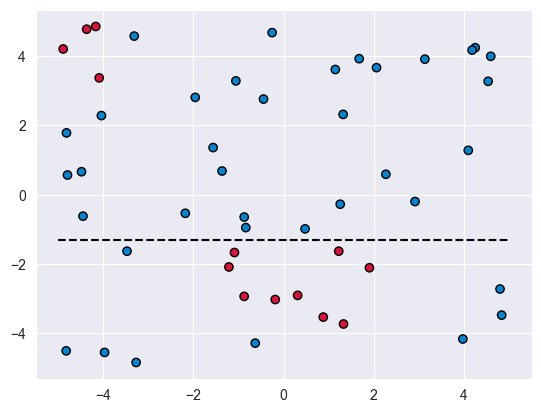
\includegraphics[height=0.3\textheight]{../../Images/decision_stump.png}
\end{frame}

%%%%
\begin{frame}
    \frametitle{Construction}
Given sample data, $\mathcal S = \{(\x_i, \ix y_i)\}_{i=1}^n$ with $\x_i\in\mathbb R^d$, the decision stump which is the best fit may be found simply by minimizing error {--} that is, find the values of $b, \theta$, and $j$ that achieves the highest accuracy on $\mathcal S$. 

If there is no point $\x_i$ between $\{x_{i,j} = b\}$ and $\{x_{i,j} = b'\}$, then the accuracy for $(b,\theta,j)$ and $(b',\theta,j)$ are the same. So, one can consider just values of $b$ that are an average of two ``consecutive'' $x_{i,j}$ (and one less than all such $j^{th}$ coordinates, and one larger than all of them). This gives a finite set of decision stumps to check.

A naive algorithm to determine the most accurate among this finite set of decision stumps takes on the order of $dn^2$ operations. 

However, there is a more efficient approach, taking only $dn\log(n)$ time.
\end{frame}

%%%%
\begin{frame}
    \frametitle{Construction of a decision tree}
A decision stump is a decision tree with ``depth'' 1. That is, can think of a decision tree as a collection of nested decision stumps, on smaller and smaller subsets of the data.

Begin with a decision stump on all the data; i.e., find a hyperplane $ x_j = b$, where $ 1\le j\le d$ and $b$ is some number and each data point is on one side: for each $\x_i \in \mathcal S$, either $x_{i,j} < b$ or $ x_{i,j} > b$. This partitions the data into two subsets.

How do you choose where to make a split? You could use the highest accuracy approach described for stumps, but this has disadvantages when the proportion of $\ix y_i$ that are positive, compared to negative, are unbalanced.

Often, something called \textbf{Information Gain} is used, which is defined via an entropy function $e$. That is, set $e(r) = -r\log(r) - (1-r)\log(1-r)$. Now, before making a split, set $r$ to be the proportion of $\ix y_i$ that are $1$ and $m$ the number of points. 

Next, define $r_+$ (resp.\ $r_-$) to be the proportion of points on the positive (resp.\ negative) side of the split that will have label $1$, and let $m_+$ (resp.\ $m_-$) be the numbers of points on the positive (resp.\ negative) side. The information gain of the split is 
    \[e(r) - (\frac{m_+}{m}e(r_+) + \frac{m_-}{m}e(r_-)).\]

\end{frame}

%Often when decision trees are discussed, the data is converted to points which have binary coordinates (either 0 or 1); however, it is not necessary. Here I will discuss data points with \( d\) numerical coordinates, in \( \mathbb R\), as I have before.  If you wish, you can translate to the binary setting by using 0 or 1 to represent whether or not the given data is larger than some threshold in each coordinate.

%%%%
\begin{frame}
    \frametitle{Multiple branches}
The goal of the process is to recursively partition each side. On each step, one chooses the split with maximum Information Gain, at each step restricting to the two subset of data points on one side. The process ends when points in the same part have the same label, or until some predetermined depth is reached. 

An innermost region (where points have the same label) corresponds to a \textbf{leaf} of the tree.

\centering 
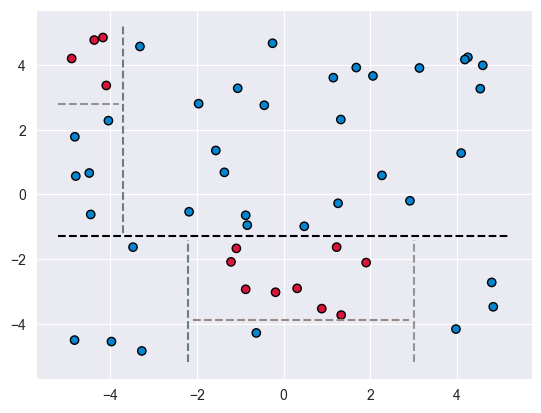
\includegraphics[height=0.35\textheight]{../../Images/decision_tree.png}
\end{frame}

%Below is a potential set of data for binary classification, with only 4 negatively-labeled points (the red points). If the first split made is along the horizontal line \( x_2 = -1.8\) (so \( j = 2\) and \(b = -1.8\)), then all but one point above the line is blue and 3 of the 12 points below the line are red.

%[gallery columns="2" size="medium" ids="948,949"]

%Call the top region above the line the positive region of the split; below the line is the negative region. Continuing with nested splits into each side, one could imagine using two more splits in the positive region to isolate the one red point. A way to isolate the three red points in the negative side is with three additional nested splits on that side (see the figure below).

%I have drawn the corresponding decision tree to the right, where the dashed lines in the figure correspond to branchings of the tree. The branches of the tree are labeled with + or -, corresponding the side of the line one is following (in each split for <em>this</em> tree, the negative side is the one side that contains red points).

%[gallery columns="2" size="medium" ids="950,952"]

% Each leaf of the tree is a node where there are no further splittings beyond it, labeled by the labels of points in that region. The <strong>depth</strong> of a decision tree is defined to be the maximal number of branches that can be followed from the top node to a leaf. So the depth of the example decision tree is 4.

%%%%
\begin{frame}
    \frametitle{Decision tree model}
    Start by determining a decision tree on training data, as above. Then, given test data (not yet "seen" by the model), the decision tree model will check in which partition the test point resides. Then, it labels the test point with the label of the corresponding leaf. 
    
    Often (to avoid overfitting), you decide beforehand on the depth of the tree (the maximal number of splits to get to a leaf). Since this will result in having more than one label in some of the partitions (and possibly all), the label given to a test point in each leaf is a function of the training labels in that partition {--} if the goal is classification, with some categorical labels, the label that has majority; if the goal is regression, with numerical labels, the mean, or the median, could be used.
\end{frame}


% Now, to define \( IG\) of a split, first let \( r = {\bf P}(y=1)\), the probability that the label is 1 (in the particular subset you have restricted to <em>before</em> the split). Let \( m\) be the number of points under consideration. In our example above, and <em>after</em> the first split along \( x_2 = -1.8\) was made, say we are in the positive side where there is 1 red point (negatively labeled), and are trying to figure out where to make the second splitting. Then \( m = 38\) (there are \( 38\) points above the horizontal line), and \(r = 37/38\).

% Next, for a potential splitting, let \(r_+ = {\bf P}(y=1\ |\ x\text{ on the + side})\) be the fraction of blue (+1 labeled) points on the positive side of that split. Similarly, define \(r_- = {\bf P}(y=1\ |\ x\text{ on the - side})\). Also, let \( m_{\pm}\) be the total number of points on each side. In the continuing example, say the potential split is along the line \( x_1 =-3.9\) (one of the second level splits depicted in the figure above). Then \(r_+ = 35/35 = 1\) and \(r_- = 2/3\).

% Now, with \(r, r_+,\) and \(r_-\) defined, the information gain of a split \( s\) is \( IG(s) = e(r) - (\frac{m_+}{m}e(r_+) + \frac{m_-}{m}e(r_-))\). Note that it actually doesn't matter which side of the line is the positive or negative side, just where the splitting line is. For the continuing example, the information gain is
% <p style="text-align: center;">\( e(37/38) - (\frac{35}{38}e(1) + \frac{3}{38}e(2/3)) \approx 0.07.\)</p>
% If you were to use \( IG\) to build a decision tree, then at each step you must find the split, on the subset of the data under consideration, that has maximal information gain.

% <sup id="footnote4">4.</sup> <span style="color: gray;">It is important to consider this a definition, not a consequence of the logarithmic expression given above. While you can get \( 0\) from <em>a limit</em> of that expression as \( r\to 0^+\), it is <span style="text-decoration: underline;">not</span> equal to its value. Trying to say it is might not lead to trouble if you only think this way for the purpose of the calculation of a single entropy function value. However, if you attempt to do any arithmetic and use properties of logarithms, thinking of \( 0\log 0\) as being equal to \( 0\) will easily lead to statements like \( 1 = 2\).</span>

% <sup id="footnote5">5.</sup> <span style="color: gray;">The logarithm function can have any base. Most of the time, in discussions of Information Gain, the base is 2 due to the area of study that the idea comes from.</span>

\section{Clustering}

\begin{frame}
    \frametitle{What is clustering?}
\end{frame}

\begin{frame}
    \frametitle{Applications of clustering}
\end{frame}

\begin{frame}
    \frametitle{K-means}
\end{frame}

\begin{frame}
    \frametitle{DBSCAN}
\end{frame}

\end{document}